\documentclass[12pt,oneside]{book}

% --- Encoding & fonts for pdfLaTeX ---
\usepackage[utf8]{inputenc}
\usepackage[T1]{fontenc}

% Page & typography
\usepackage[a4paper,margin=1in]{geometry}
\usepackage{microtype}
\usepackage{setspace}
\onehalfspacing
\usepackage{graphicx}
\usepackage{booktabs}
\usepackage{amsmath,amssymb}
\usepackage{xcolor}
\usepackage{braket}
\usepackage{ctex}
\usepackage{hyperref}

% Colors
\definecolor{BrandBlue}{HTML}{0B5FFF}
\definecolor{BrandBlueLight}{HTML}{EAF1FF}
\definecolor{BrandRed}{HTML}{B22222}
\definecolor{BrandRedLight}{HTML}{DC143C}
\definecolor{BrandGreen}{HTML}{228B22}
\definecolor{BrandGreenLight}{HTML}{90EE90}
\definecolor{RefGray}{HTML}{555555}
\definecolor{RefGrayLight}{HTML}{F5F5F5}
\definecolor{RefBrown}{HTML}{8B5A2B}
\definecolor{RefBeige}{HTML}{FAF3E0}

% contents
\usepackage{titletoc}
\titlecontents{chapter}
  [1.5em]{}{\contentslabel{1.5em}}{}{\hfill\contentspage}[]
\titlecontents{section}
  [3.0em]{}{\contentslabel{2.0em}}{}{\hfill\contentspage}[]

% Chapter styling
\usepackage{titlesec}
\titleformat{\chapter}{\normalfont\LARGE\bfseries}{\color{BrandBlue}\thechapter}{1em}{}
\titlespacing*{\chapter}{0pt}{-2pt}{18pt}

\ctexset{
  contentsname = Contents,
  listfigurename = List of Figures,
  listtablename = List of Tables,
  figurename = Figure,
  tablename = Table,
  indexname = Index,
  bibname = References,    % report/book 类
  appendixname = Appendix,
  proofname = Proof
}

% Boxes
\usepackage[skins,breakable]{tcolorbox} %
\tcbset{
  arc=4pt,              
  drop shadow,         
  boxrule=2pt,
  breakable,
  left=10pt,right=10pt,top=8pt,bottom=8pt,
}
\newtcolorbox{bluebox}[1][]{title=#1, colframe=BrandBlue,  colback=BrandBlueLight}
\newtcolorbox{redbox}[1][]{title=#1,  colframe=BrandRed,   colback=BrandRedLight!15}
\newtcolorbox{greenbox}[1][]{title=#1,colframe=BrandGreen, colback=BrandGreenLight!25}

% for book icon
\usepackage{fontawesome5}

\newtcolorbox{referencebox}[1][]{title={\textcolor{white}{\faBook\ References}},
  colframe=RefBrown,
  colback=RefBeige,
  coltitle=black,
  fonttitle=\bfseries,
  arc=4pt,
  drop shadow,
  boxrule=2pt,
  breakable,
  left=10pt,right=10pt,top=8pt,bottom=8pt,
}

% Hyperref should be loaded before bookmark
\usepackage{hyperref}
\hypersetup{
  colorlinks=true,
  linkcolor=blue!60!black,
  urlcolor=blue!60!black,
  citecolor=blue!60!black
}
\usepackage{bookmark}

% --- Cover with centered logo ---
\usepackage{tikz}
\newcommand{\makeModernCover}{
\begin{titlepage}

  \vspace*{3cm}
  \begin{center}
    {\Huge\bfseries Quantum 101:\par}
    \vspace{0.8cm}
    {\large A Beginner's Journey into Quantum Computing\par} % 用直撇号,避免编码问题

    \vspace{2.5cm}
    
\includegraphics[width=0.35\textwidth]{LogoWithText.pdf} % 确保文件存在 (pdf/png/jpg)

    \vspace{2.5cm}
    {\Large \textbf{Zhehao Yi}\par}
    \vspace{0.2cm}
    {\large September 12. 2025\par}
  \end{center}
  \vfill
\end{titlepage}
}

\begin{document}

\makeModernCover
\frontmatter
\tableofcontents
\mainmatter

\chapter{Perface}
Before we begin our journey into quantum computing, let's pause and think about two simple questions: What is quantum? and What is computing?

At first, these questions may sound easy, you might even feel you already know the answers. But don't be in a hurry! The most important things you'll need at the start are curiosity and creativity. Once you allow yourself to imagine, the quantum world becomes less intimidating, and real understanding begins to grow, not just the kind of knowledge you memorize for a test.

In the world of quantum computing, there are really just two things you need to grasp: what it is and what it can do. That's it. Our journey will start with the simplest symbols, then move on to basic quantum algorithms, simple quantum circuits, and finally a small quantum computing project we'll build together. (Sounds exciting?)

Along the way, we'll also touch on some of the most important Python tools, such as PyTorch, TensorCircuit, TorchQuantum, and NumPy. If anything feels unclear, don't worry: you can always check the official documentation for more details.

The references for this document are as follows:
\begin{referencebox}[Reference]
  \begin{itemize}
    \item \textit{Nielsen, M. A., \& Chuang, I. L. 2010. Quantum Computation and Quantum Information: 10th Anniversary Edition. Cambridge: Cambridge University Press.}
    \item \textit{Cohen-Tannoudji, C., Diu, B. and Laloe, F., 1986. Quantum mechanics, volume 1. Quantum Mechanics, John Wiley \& Sons.}
    \item \textit{姚 珩. 2018,「量子力學」, 滄海書局, 1-491頁。}
    \item \textit{TensorCircuit: \href{https://tensorcircuit.readthedocs.io/en/latest/}{https://tensorcircuit.readthedocs.io/en/latest/}}
    \item \textit{TorchQuantum: \href{https://hanruiwanghw.wixsite.com/torchquantum}{https://hanruiwanghw.wixsite.com/torchquantum}}
    \item \textit{PyTorch: \href{https://pytorch.org/}{https://pytorch.org/}}
  \end{itemize}
\end{referencebox}

To be honest, don't be scared by the name ``quantum computing." It's not as difficult as it sounds! You might be thinking: ``But I don't have a background in quantum mechanics or advanced mathematics.” Don't worry! All you really need is some basic linear algebra. If you do know a bit of quantum mechanics, that's fantastic, but it's by no means required. We'll keep things as simple as possible.

If you've read this far, it means you're curious about quantum computing, and that's the only thing you truly need. So thank you for joining! Now, Warriors, grab your armor and sword - your laptop and a piece of paper - and get ready to step into a whole new world.

Welcome to Quantum Computing. Let's make this journey fun!

\vspace{2em}
\textbf{Zhehao Yi}

AI, Autonomy, Resilience, Control Lab (AARC Lab)

Department of Electrical and Computer Engineering

The University of Alabama in Huntsville

Huntsville, AL 

United States

September 12, 2025

\chapter{Basic Quantum Mechanics}
Imagine tossing a coin into the air. While it spins, it is not simply ``heads" or ``tails", in some sense, it is both at the same time. Only when it lands in your hand do you see a definite result. This simple image captures the spirit of quantum mechanics: a world where particles can exist in multiple states at once, and where observation itself plays a role in shaping reality.

In this chapter, we will use everyday analogies like this to introduce the core ideas of quantum mechanics, such as superposition, uncertainty, and entanglement. No complicated math, just the essential intuition you'll need to understand how quantum mechanics gives birth to quantum computing.
\section{Why Quantum?}
Every day, we're secretly doing physics experiments without even noticing. When you lug that heavy Amazon package up six flights of stairs, you’re working against gravity. When you launch a basketball toward the hoop, you’re creating a perfect parabolic arc (at least in theory). And when you drive from Huntsville to Atlanta, your car is constantly playing with speed, acceleration, and friction. All of these everyday adventures are ruled by classical mechanics. And at the core of it all stand Newton’s three legendary laws of motion, the ultimate ``rules of the game" for how things move.

\begin{bluebox}[Newton's Law of Motion ]
  \begin{enumerate}
    \item A body remains at rest, or in motion at a constant speed in a straight line, unless it is acted upon by a force.
    \item At any instant of time, the net force on a body is equal to the body's acceleration multiplied by its mass or, equivalently, the rate at which the body's momentum is changing with time.
    \item If two bodies exert forces on each other, these forces have the same magnitude but opposite directions.
  \end{enumerate}
  Reference: \href{https://en.wikipedia.org/wiki/Newton%27s_laws_of_motion}{Law of Motion}
\end{bluebox}

We have drawn a simple diagram of Newton's three laws in Figure. \ref{fig:newton}, hoping that this will help you recall some classic parts.


\begin{figure}[htbp]
    \centering
    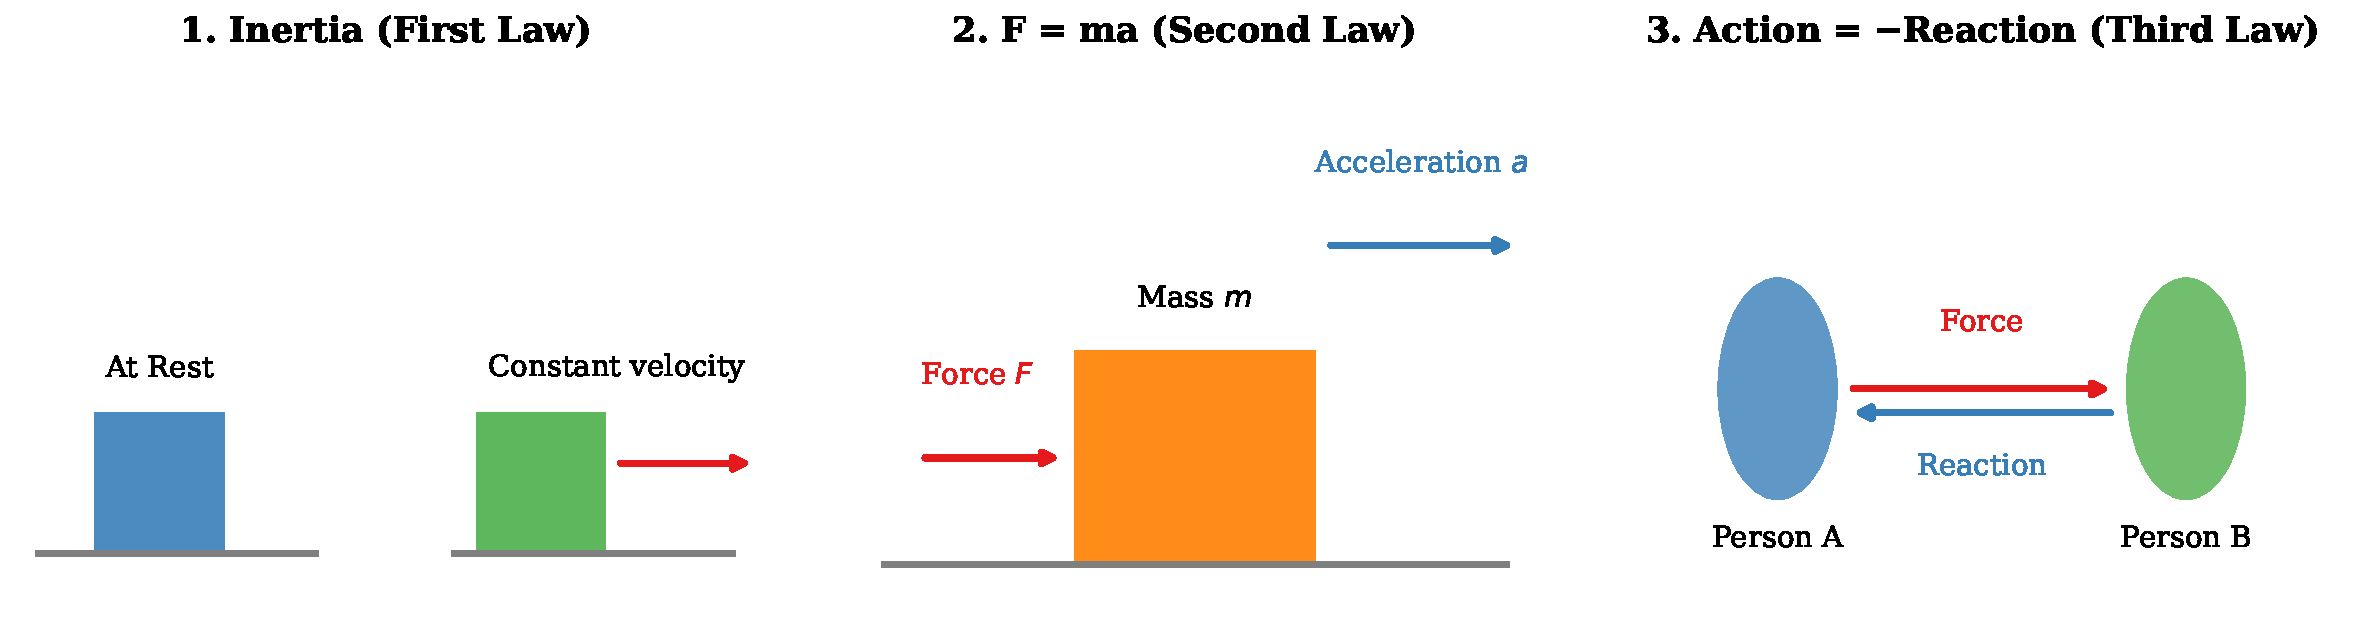
\includegraphics[width=1\linewidth]{newton_three_laws_nature_style_v3.pdf}
    \caption{Illustrations of Newton's three laws of motion.}
    \label{fig:newton}
\end{figure}

Classical mechanics has served us well, even if only to figure out how to open a can of Spam. More importantly, ever since Sir Isaac Newton, while resting under an apple tree, was struck by a falling apple and conceived the law of universal gravitation, 
\begin{bluebox}[Newton's law of Universal Gravitation]
  Newton's law of universal gravitation describes gravity as a force by stating that every particle attracts every other particle in the universe with a force that is proportional to the product of their masses and inversely proportional to the square of the distance between their centers of mass.
  \begin{equation*}
    F = G \frac{M_{1}M_{2}}{r^2}
  \end{equation*}
  Reference: \href{https://en.wikipedia.org/wiki/Newton%27s_law_of_universal_gravitation}{Universal Gravitation}
\end{bluebox}
our understanding of the world has been transformed. We no longer limit ourselves to studying how cars drive on roads or how balls arc through the air; instead, we set our sights on the sky above and reach outward to explore the universe.
\section{Core Ideas of Quantum Mechanics}

\section{Thought Experiments}

\section{From Quantum Mechanics to Qubits}

\section{Summary \& Transition}

\chapter{Test}
\begin{bluebox}[Info]
Blue box works.
\end{bluebox}

\begin{redbox}[Warning]
Red box works.
\end{redbox}

\begin{greenbox}[Example]
Green box works. Also $\braket{0|1}=0$.
\end{greenbox}

\end{document}
